\documentclass{article}

% Use the appropriate workshop option once anonymity requirements are confirmed.
% \usepackage[dblblindworkshop]{neurips_2026}
\usepackage[sglblindworkshop]{neurips_2026}

\usepackage[utf8]{inputenc}
\usepackage[T1]{fontenc}
\usepackage{hyperref}
\usepackage{url}
\usepackage{booktabs}
\usepackage{amsmath}
\usepackage{amsfonts}
\usepackage{microtype}
\usepackage{xcolor}
\usepackage{graphicx}
\usepackage{subcaption}
\usepackage{multirow}

\graphicspath{{../results/figures/}}

\title{Where Code Models Build Program Semantics, and What Breaks It}

\workshoptitle{Interpretability as a Science}

\author{
  Virginia Ceccatelli \\
  University College London \\
  \texttt{v.ceccatelli@ucl.ac.uk}
  \And
  Lorenzo Cavallaro \\
  University College London \\
  \texttt{l.cavallaro@ucl.ac.uk}
}

\begin{document}

\maketitle

\begin{abstract}
Code language models can appear to understand programs while only exploiting identifier spelling, proximity, and indentation, all of which correlate with program meaning. Distinguishing the two requires a baseline that is \emph{fixed by construction} rather than estimated. We build one: pairs of Python programs that are identical except for a single character, chosen so that the character changes which definition a variable use refers to while leaving every surface cue around both probing sites untouched. Any feature of the text is therefore uninformative by construction, and a model-free baseline scores exactly 0.500 rather than approximately so. Against that floor, in DeepSeek-Coder 1.3B and 6.7B, variable binding is absent at the input, is constructed within the first few transformer blocks, plateaus near 0.984 in the middle of the network, and is partly shed before the output; def--use structure follows the same profile. Stressing the representation separates what it is made of from what it merely correlates with: renaming every identifier drives the earliest layers below chance while middle layers hold at 0.85--0.90, and a thousand tokens of inert filler costs almost nothing (0.921) where scope-shadowing filler of the same length reduces the same probe to chance. What breaks the representation is added semantic difficulty, not added distance or altered spelling. Finally we ask whether the model's own computation reads the value it has resolved, by exchanging two output-aligned coordinates at a position where the two programs are token-identical. Against a dose-matched control that pushes along the true counterfactual direction, the answer depends sharply on where one intervenes: at the readout position the exchange reaches 46\% of an ideal same-norm edit while two matched-norm controls reach zero, and it moves each downstream operation toward its own different answer; at the site where the binding is resolved, the state's response to small edits is so nonlinear that even an ideal edit of that size does nothing, so the question is underpowered rather than answered. The causal channel we find is output-aligned value directions in general, not the Jacobian-corrected lens, which the plain unembedding matches or beats throughout.
\end{abstract}

\section{Introduction}
\label{sec:introduction}

Code language models predict convincing programs, but this does not establish that they compute the relations that determine program meaning. Equal names usually denote the same variable, definitions and uses are usually nearby, and indentation usually exposes control structure. A probe that recovers binding, data flow, or control dependence from a model's hidden states may therefore be recovering the model's computation --- or it may be recovering the text, which the hidden states also contain.

The usual response is to estimate how much a shortcut could explain and subtract it. We take a different route, available in code and rarely available elsewhere: make the shortcut carry \emph{no information at all}, by construction. Consider two programs that differ in one character:

\begin{center}
\begin{minipage}{0.30\linewidth}
\begin{verbatim}
x = 3
def f():
    y = 7
    return x
\end{verbatim}
\end{minipage}
\hspace{0.06\linewidth}
\begin{minipage}{0.30\linewidth}
\begin{verbatim}
x = 3
def f():
    x = 7
    return x
\end{verbatim}
\end{minipage}
\end{center}

The marked use is the same token at the same index in both. On the left it refers to the outer definition; on the right the inner line has captured the name, so it refers to that instead. Both values occur in both programs, the token windows around both probing sites are identical, and the distance between them is unchanged. The correct answer flips; nothing observable about the text does. A model-free baseline therefore scores exactly $0.500$ --- not approximately, but as a property of the construction --- and so does a probe on the context-free embedding layer. Everything above that floor is something the model computed.

We use this leverage for three questions, in increasing strength. Is the relation \emph{built}, and where? What is it \emph{made of} --- which perturbations destroy it and which leave it intact? And is it \emph{used}: does the model's own downstream computation read the relation it has computed, or merely coexist with it?

Prior work shows that code-model representations preserve AST structure and expose identifiers, namespaces, data flow, control flow, and data dependence \cite{wan2022capture,hernandez2022astprobe,troshin2022probing,ma2024unveiling}, and that models trained on programs can acquire latent execution state \cite{jin2024emergent}. These results establish recoverability. Recoverability alone does not separate model computation from surface cues or from what the probe itself learned \cite{hewitt2019control}, and it does not establish causal use. We connect probing to activation patching \cite{zhang2023patching} and to output-aligned readouts of internal state \cite{gurnee2026workspace}.

Our contribution is fourfold. First, binding and def--use structure are absent from the input representation and constructed within the first transformer blocks, replicated across two model scales at the same relative depth. Second, the representation has a characterizable failure surface: it is robust to distance and to identifier renaming in the middle layers, and it collapses under scope shadowing and under control-flow flattening --- it breaks when the underlying problem gets harder, not when the text gets longer or is spelled differently. Third, a two-coordinate exchange at a token-identical position shows the resolved value is causally reused near the output, specifically and in an operation-appropriate way, but attributes it to output-aligned value directions rather than to the Jacobian-corrected readout we built to find it. Fourth, and methodologically: the same intervention at the site where binding is resolved returns a clean-looking null that a dose-matched control shows to be underpowered, which is a general hazard for low-rank interventions and one we would have published without that control.

\section{Setup and Controls}
\label{sec:setup}

We study frozen DeepSeek-Coder models at 6.7B parameters (main) and 1.3B parameters (cross-scale replication). The synthetic Python corpus contains binding, shadowing, control-dependence, and source--propagation--sanitizer--sink programs. The generator records exact semantic graphs; AST spans are mapped to tokenizer offsets and checked against the original source. Def--use ground truth is independently cross-checked against Beniget. Linear probes use five-fold cross-validation grouped by source program and are reported with within-program shuffled-label selectivity.

The experiments are organized around controls that make each claim falsifiable (Table~\ref{tab:controls}). Context-matched binding pairs differ by one binding-changing character while preserving the probe anchors, placing both the model-free surface baseline and context-free embedding layer at exactly 0.500. Def--use negatives are distance-matched, and control-dependence negatives occur under a sibling guard at the same indentation depth. Frozen probes are evaluated under added context and execution-verified obfuscations without retraining. Behavioral and lens nulls are reported only with controls showing that the instrument works at the same decision point.

\begin{table}[t]
  \centering
  \small
  \caption{Each claim is paired with a construction that could falsify it.}
  \label{tab:controls}
  \begin{tabular}{p{0.34\linewidth}p{0.58\linewidth}}
    \toprule
    Claim & Falsifying construction \\
    \midrule
    Relation computed, not read from surface & Token-matched pairs with a label flip; surface floor exactly 0.500 \\
    Probe reads the state, not its own labels & Retrain on labels shuffled within each source program; report the difference \\
    Robustness result is not probe re-fitting & Probes frozen before any variant is generated; ground truth rebuilt per variant \\
    Degradation is semantic, not positional & Filler types matched on token count, varied only in whether they interfere with scope \\
    A null reflects the model, not a dead instrument & A positive control of the same kind, at the same site, on the same states \\
    Intervention changed the relation, not the input & Intervene only at positions where the two programs are token-identical \\
    \bottomrule
  \end{tabular}
\end{table}

The last two rows are the ones this paper had to learn. An earlier version of this work reported two null results that we have since withdrawn, because their positive controls were of the wrong kind to license the reading we gave them, and one causal result whose intervention site was the one place the two programs differed. Appendix~\ref{app:retired} documents all three, since a controls-focused venue should see the failures as well as the survivors.

Full generation, alignment, probe, and intervention details are provided in the supplementary material. The main text retains the controls required to interpret each claim.

\section{The Representation Is Built With Depth}
\label{sec:built}

Figure~\ref{fig:binding} is the paper's central measurement. On context-matched binding pairs, the model-free surface baseline and the context-free embedding layer both sit at exactly 0.500. The first transformer block reaches 0.53--0.57, layer 3 reaches 0.91--0.96, both models peak near 0.984 in the middle layers, and accuracy falls back to about 0.92 at the final layer.

Read as a curve, this has three phases, and each says something different. \emph{Nothing at the input}: the relation is not in the tokens, so it cannot be looked up --- it has to be computed. \emph{Rapid construction}: most of the work happens in the first few blocks, which is early for a relation that requires resolving a scope. \emph{Partial shedding near the output}: the final third of the network gives some of it back, which is what one expects if an abstract fact is used and then displaced by the concrete business of predicting the next token. Def--use edges follow the same profile, reaching approximately 0.99, with only mild decay when the definition and the use are 50--200 tokens apart.

Two features of this curve are worth separating from the headline number. The two model scales agree on shape and differ only where a scaling account predicts: the larger model does slightly less of the work in block 0 and holds its peak over a longer stretch --- the same relative depth, stretched. And the surface and embedding rows are numerically identical across the two models, which they must be, since neither involves the model; that identity doubles as a check that both runs share the same ground truth.

\begin{figure}[t]
  \centering
  \begin{subfigure}[t]{0.49\linewidth}
    \centering
    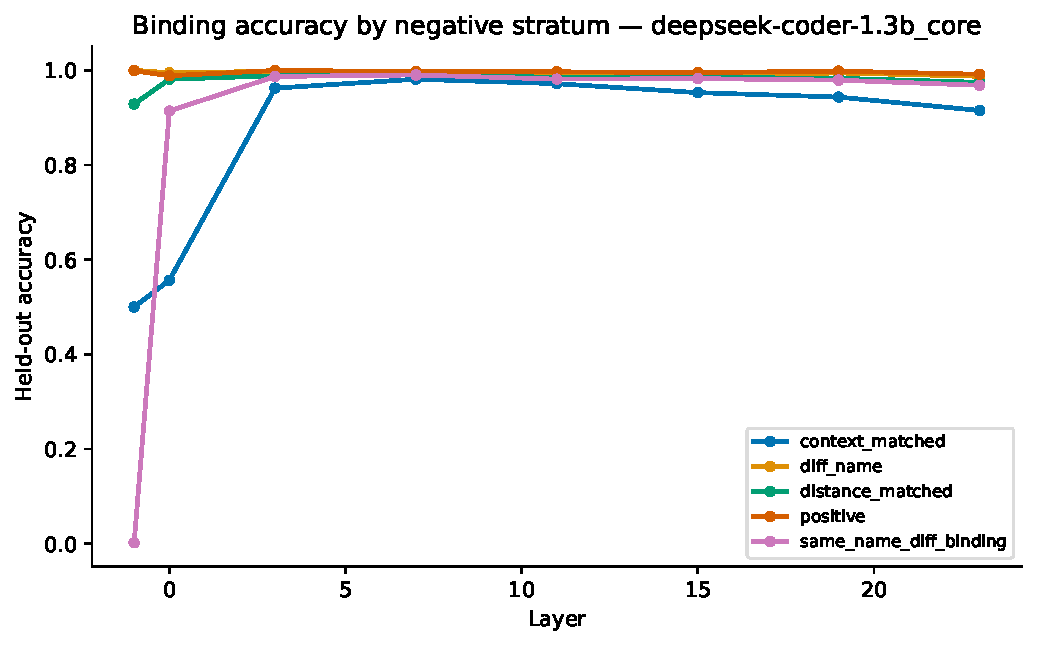
\includegraphics[width=\linewidth]{binding_strata_deepseek-coder-1.3b_core.pdf}
    \caption{DeepSeek-Coder 1.3B.}
  \end{subfigure}
  \hfill
  \begin{subfigure}[t]{0.49\linewidth}
    \centering
    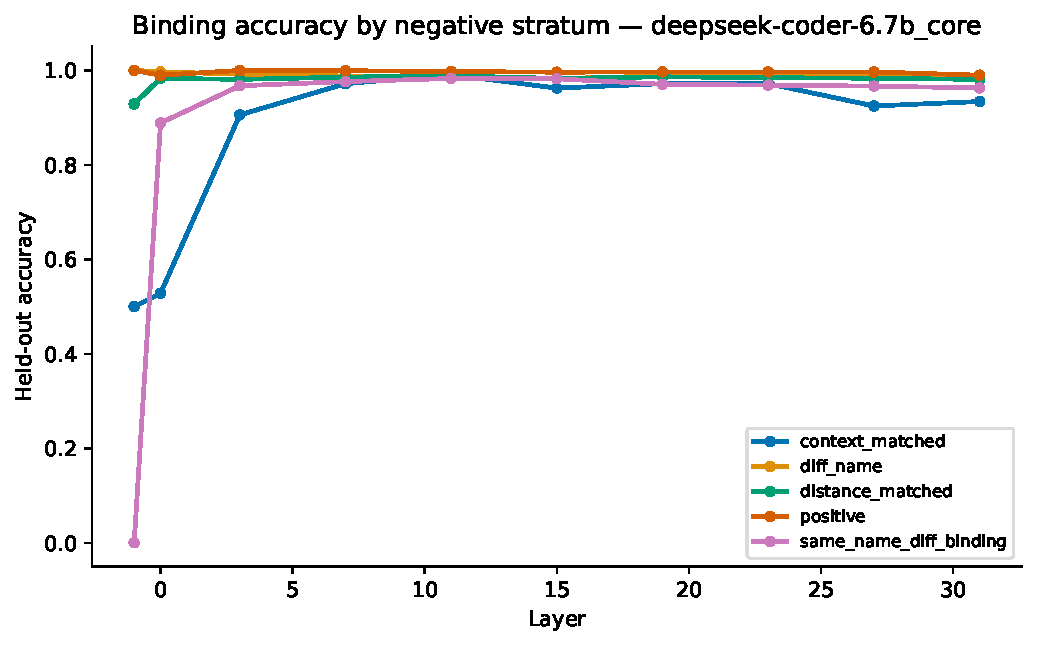
\includegraphics[width=\linewidth]{binding_strata_deepseek-coder-6.7b_core.pdf}
    \caption{DeepSeek-Coder 6.7B.}
  \end{subfigure}
  \caption{Binding by layer and negative stratum. The context-matched relation rises from exact surface and embedding floors of 0.500 to approximately 0.984 in middle layers, replicated across model scale.}
  \label{fig:binding}
\end{figure}

\section{What the Representation Is Made Of}
\label{sec:robustness}

Knowing the relation is computed does not say what it is computed \emph{from}. We answer that by breaking it in controlled ways. Probes are fitted once, on the base programs, and then frozen: they are never refitted on a perturbed variant, so any change in accuracy is a change in the model's state rather than in the probe. Ground truth is recomputed from each variant's own source, so a perturbation that genuinely changes the answer is scored against the new answer.

\paragraph{Distance is cheap; interference is not.}
We insert filler between the tracked definition and use, sized by real tokenizer counts, and vary only what the filler \emph{does}. At 500 inserted tokens, 6.7B binding accuracy is 0.921 under inert prose but 0.570 under filler that reuses the tracked names; at 1{,}000 tokens the latter reaches chance while every other filler type stays above 0.70. A thousand tokens of comments is nearly free. The same length of code that forces a genuine scope resolution destroys the representation. Per layer, the pattern sharpens: under scope shadowing, block 0 is the most stable part of the network and the middle layers --- the ones doing the binding work --- are the ones that collapse. The interference lands on the computation, not on the lookup.

\paragraph{Spelling is cheap in the middle, decisive at the edges.}
We then apply a cumulative ladder of semantics-preserving transformations, each variant execution-verified to behave identically to its base. Renaming every local identifier is the first cliff, and averaging over layers hides what it means: at the embedding and block-0 layers renaming pushes the probe \emph{below} chance (0.29--0.33), because those layers keyed on the identifier strings and renaming actively misleads them, while layers 7--15 hold at 0.85--0.90. That contrast is the paper's cleanest statement of the lexical/structural split: early layers carry names, middle layers carry something closer to the relation. Opaque predicates and rewritten arithmetic barely register, because they do not change which definition reaches which use. Control-flow flattening is the real boundary: once the control structure is dissolved into a dispatch loop, even the best layer reaches only about 0.75.

Taken together, the two ladders describe one failure surface. The representation is robust to how far apart things are and to what they are called, and it fails when the scope or control structure it is a representation \emph{of} becomes harder. That is what one wants from a computed relation rather than a positional heuristic --- and it is also a first, coarse map of when a tool built on these representations should not be trusted.

\section{Is the Relation Used? Where, and How Much}
\label{sec:causal}

Everything above is correlational. A representation can be a faithful shadow of a computation that happens elsewhere, and probing cannot tell the difference. The question that matters for using these representations downstream is whether the model's own computation reads what it has built.

\paragraph{What we can show.}
We patch hidden states from a clean program, which passes a sanitized value to a sink, into a token-aligned corrupted program that passes the raw value. In 6.7B, recovery at the sink-argument token is approximately 0.99 at layer 0 and declines with depth, while recovery at the final position rises to 1.00 at layer 31 (Figure~\ref{fig:patching}). The smaller model shows the same crossover at compressed depth. This is a reproducible description of \emph{where the decision becomes committed}: early, the answer is determined at the argument; late, it is determined at the readout position, and the crossover sits near where the binding curve plateaus.

\begin{figure}[t]
  \centering
  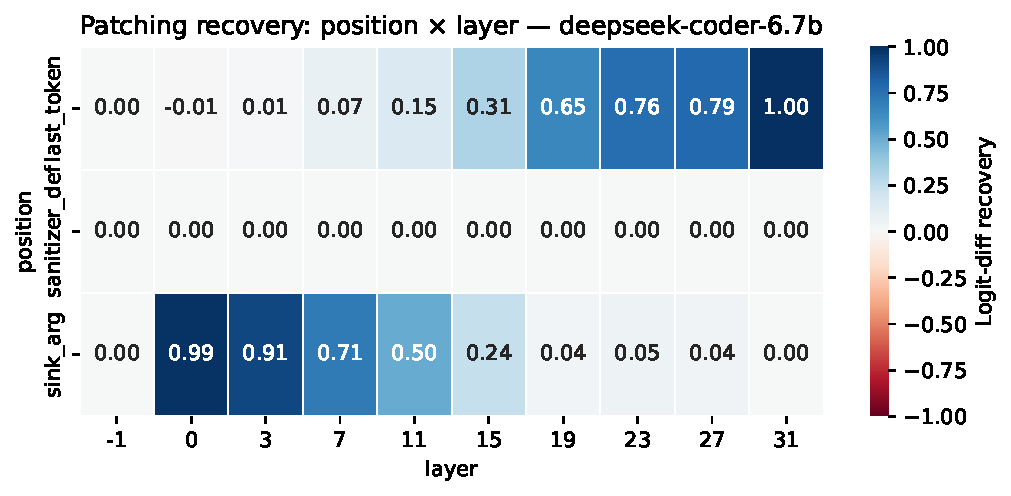
\includegraphics[width=0.68\linewidth]{patching_recovery_deepseek-coder-6.7b.pdf}
  \caption{Activation-patching recovery in DeepSeek-Coder 6.7B. Causal influence moves from the sink argument in early layers to the final position in late layers. Patching the sanitizer definition recovers 0.000 at every layer.}
  \label{fig:patching}
\end{figure}

\paragraph{Why this is not yet evidence of use.}
The sink-argument token is the one place where the two programs differ --- that is how the pair is built. Patching it transports the surface difference along with whatever semantic state the position holds, and this design cannot separate them; near-perfect recovery at layer 0 is exactly what pure input restoration would produce. The sanitizer-definition position recovers 0.000 at every layer, but with no positive control at that site the zero is an absence of evidence at one hand-picked token. And recovery at the final position in late layers forces the answer trivially.

\paragraph{A targeted intervention.}
We therefore built an intervention with the three properties this one lacks. It acts at a position where the two programs are \emph{token-identical}: on counterfactual pairs of the form in Section~\ref{sec:introduction}, at the marked use. It edits a nameable two-dimensional part of the state rather than replacing it: with $V=[v_{\text{src}}, v_{\text{tgt}}]$ the output-aligned directions of the two candidate values and $c = V^{+}h$ their coordinates, we set $h \mapsto h + V(\mathrm{swap}(c) - c)$, which exchanges the two coordinates and leaves the orthogonal complement untouched. And it is checked against several downstream operations over the same value, so that one edit must produce a \emph{different} correct answer in each --- something an intervention that merely pushes on the answer token cannot do.

The control that matters most is a dose-matched one, and it changed our conclusion. A two-dimensional edit moves only a few percent of the state's norm, so ``the edit did nothing'' is ambiguous between \emph{these coordinates are not read} and \emph{no edit this small moves this site}. We therefore also push along the empirical counterfactual direction $h_{\text{other}} - h_{\text{self}}$ at a sweep of doses $\alpha$; at $\alpha = 1$ this reproduces the whole-state patch exactly (verified to machine precision), so the sweep measures the site's own norm-to-effect curve instead of assuming it is linear.

\begin{table}[t]
  \centering
  \small
  \caption{Dose-matched intervention at two positions in DeepSeek-Coder 6.7B, test split, $n=204$ pairs. $\|\Delta h\|/\|h\|$ is the fraction of the state moved; efficiency is the logit shift per unit of that fraction. Brackets are cluster-bootstrap intervals over base programs.}
  \label{tab:doseresponse}
  \begin{tabular}{llrrr}
    \toprule
    Position & Edit & $\|\Delta h\|/\|h\|$ & $\Delta$ logit-diff & Efficiency \\
    \midrule
    \multirow{4}{*}{Marked use, L8}
      & Counterfactual push, $\alpha{=}0.03$ & 0.021 & \phantom{0}0.002 [$-$0.000, 0.004] & 0.08 \\
      & Counterfactual push, $\alpha{=}0.3$  & 0.214 & \phantom{0}0.069 [0.047, 0.094] & 0.32 \\
      & Counterfactual push, $\alpha{=}1$ (= whole state) & 0.713 & \phantom{0}1.066 [0.873, 1.306] & 1.50 \\
      & Value-coordinate swap & 0.037 & \phantom{0}0.002 [$-$0.000, 0.005] & 0.06 \\
    \midrule
    \multirow{5}{*}{Readout position, L24}
      & Counterfactual push, $\alpha{=}0.03$ & 0.012 & \phantom{0}0.046 [0.041, 0.052] & 3.80 \\
      & Counterfactual push, $\alpha{=}1$ (= whole state) & 0.407 & \phantom{0}1.960 [1.718, 2.237] & 4.81 \\
      & Value-coordinate swap & 0.077 & \phantom{0}0.141 [0.112, 0.170] & 1.82 \\
      & \quad control: unrelated digits, matched separation & 0.052 & $-$0.009 [$-$0.020, 0.001] & $-$0.17 \\
      & \quad control: Gram-matched random subspace & 0.024 & $-$0.000 [$-$0.002, 0.001] & 0.00 \\
    \bottomrule
  \end{tabular}
\end{table}

\paragraph{At the site where binding is resolved, the question is underpowered, not answered.}
Table~\ref{tab:doseresponse} shows why. At the marked use the site is causally potent --- replacing the whole state moves the answer 1.066 nats and flips 22\% of them --- but its dose-response is strongly convex: efficiency rises eighteenfold from the smallest dose to the largest, and a push along the \emph{known-correct} direction at 2\% of the norm produces 0.002 nats with an interval covering zero. The value-coordinate swap, at 3.7\% of the norm, produces the same 0.002. It is therefore not possible to conclude from this that the value coordinates are causally inert; no two-dimensional edit is large enough to test the question here. We withdraw the null we would otherwise have reported. Consistent with that, the unrelated-digit control at the same site is \emph{larger} than the real value swap (0.007 [0.005, 0.010]), so there is no value specificity at this position in either direction.

\paragraph{At the readout position the value is causally reused, and it is not the Jacobian correction that finds it.}
Here the dose-response is essentially linear --- efficiency stays between 3.8 and 4.8 across a thirty-threefold range of doses --- so a norm correction is meaningful, and the comparison is clean. The value swap reaches 46\% of the efficiency of an ideal same-norm push, while the two matched-norm controls reach zero: swapping two unrelated digits chosen to have the same numeric separation does nothing, and a Gram-matched random subspace does nothing. Swapping \emph{these} values moves the answer toward what the other value implies. On the two operation families this model computes reliably (Appendix~\ref{app:results}) the shift is positive in both, $+0.554$ for affine and $+0.171$ for modulus, so one edit produces each operation's own different answer rather than a single pushed token; the remaining three families are excluded because the model fails their arithmetic rather than their binding, which makes their nulls uninterpretable. What the effect is \emph{not} is a property of the Jacobian correction: the plain logit lens is more efficient at the same site (2.35 against 1.82). The causal channel is output-aligned value directions in general, not the corrected lens.

\paragraph{Outstanding.}
One planned control has not run: the identical swap in the basis of a supervised probe that demonstrably decodes the value from the same state (paired reversal 0.402 against a 0.025 floor at the marked use). At the readout position it would test whether a better-aimed two-dimensional edit recovers more of the ideal; at the marked use, given the convex dose-response, we expect it to be equally underpowered and we would report it as such.

\paragraph{One relation needs a narrower claim throughout.}
Control dependence reaches probe AUC 0.999, but its model-free surface baseline is already 0.927 --- a statement's guard is usually its nearest enclosing \texttt{if}, so token windows and distance recover most of it. Unlike binding, it has no construction that pins its floor to chance. We report it as the syntactic end of a spectrum whose semantic end is binding, and we draw no representational conclusion from it.

\section{Discussion}
\label{sec:discussion}

Binding and def--use structure are computed rather than read off the text, and the evidence is a floor fixed by construction rather than an estimate of how much a shortcut might explain. The representation has a shape: robust to distance and to spelling in the middle layers, fragile exactly where the underlying scope or control structure becomes harder. And the resolved value is causally reused, but late --- at the readout position, in output-aligned value directions, in a way that survives two matched-norm controls and moves each operation toward its own answer. Where the binding is actually resolved, we cannot say, because no edit small enough to be interpretable is large enough to register.

That last sentence is the methodological point, and we would have missed it. A two-dimensional intervention moves a few percent of a state's norm. Whether that is enough depends entirely on the site's response curve, which is not something to assume: at the readout position it is near-linear, and at the marked use it is convex enough that an edit along the \emph{true} counterfactual direction at the same magnitude also does nothing. Without the dose-matched control we would have reported a clean, well-controlled null --- positive readout control passing, four subspace controls at the same magnitude, a potent site --- and it would have been an artefact of rank. Low-rank interventions are increasingly common; we suggest a dose-response sweep along a known-effective direction should accompany them as a matter of course.

The same discipline retires three earlier claims (Appendix~\ref{app:retired}). ``Decodable'' is routinely treated as an endpoint; it is one claim among several, and the others need different evidence. Construction needs a floor pinned by design. Use needs an intervention at a site where the inputs agree, at a magnitude the site can register. An informative null needs a positive control \emph{of the same kind} at the same site --- and, as we learned here, at the same scale.

The limitation that most constrains the work is also what makes the testbed useful. Probes transfer to real Python at approximately 0.90 accuracy and 0.98 AUC, but natural identifiers are genuinely informative, so the embedding layer starts high and no stratum pins the floor to chance. The isolation result therefore rests on controlled programs. Building the same one-character mutation in real functions is the obvious next step and does not require the surrounding program to be statically resolvable --- which also points at where these representations would earn their keep: not on programs a parser already handles exactly, but on the dynamic constructs where it cannot.

The honest summary is narrower than the one we set out to write, and different in kind. Code models build a representation of program structure that no surface feature explains, within the first few blocks, and hold it through the middle of the network. They read a resolved value out of output-aligned coordinates near the point of use of that value --- not at the point where it was resolved, and not through the corrected readout we built for the purpose. Where the resolution itself happens, the causal question remains open for a reason we can now state precisely rather than gesture at.

\clearpage
\appendix

\section{Additional Results}
\label{app:results}

This appendix reports results that support the main argument but are not required to follow it, followed by the analyses we have withdrawn. All values are taken from the CSV files in \texttt{results/tables}; the corresponding generated figures are in \texttt{results/figures}. We distinguish aggregate results, which combine all held-out examples, from hard-stratum results, which isolate a specific shortcut. Accuracy is the fraction classified correctly. AUC is threshold-independent binary ranking performance. Selectivity is target-label accuracy minus accuracy after labels are shuffled within each source program. Recovery is the fraction of the clean--corrupted answer-logit gap restored by activation patching.

\subsection{Static probes and natural-code transfer}

Table~\ref{tab:static-probes} gives the aggregate probe results for the main model. The task-specific controlled comparisons in the main text remain more informative than aggregate accuracy: for example, aggregate binding accuracy includes easy different-name negatives, whereas the context-matched stratum removes that cue entirely. The lexical task is included only as an extraction sanity check. Its AUC is omitted because the task is multiclass.

\begin{table}[h]
  \centering
  \small
  \caption{Aggregate static-probe results for DeepSeek-Coder 6.7B. ``Control acc.'' is accuracy after within-program label shuffling. Source: \texttt{static\_probes\_deepseek-coder-6.7b\_core.csv}.}
  \label{tab:static-probes}
  \begin{tabular}{lrrrrr}
    \toprule
    Task & Best layer & Accuracy & AUC & Selectivity & Groups \\
    \midrule
    Binding & 0 & 0.975 & 0.998 & 0.391 & 423 \\
    Def--use & 3 & 0.990 & 0.999 & 0.409 & 607 \\
    Control dependence & 31 & 0.973 & 0.996 & 0.388 & 289 \\
    Taint state & 0 & 1.000 & 1.000 & 0.522 & 200 \\
    Lexical token type & 0 & 1.000 & --- & 0.843 & 347 \\
    \bottomrule
  \end{tabular}
\end{table}

Table~\ref{tab:real-code} shows that the binding and def--use decoders transfer to CodeSearchNet with nearly identical results across model scales. This rules out a pure generator-template explanation. It does not reproduce the exact semantic identification of the synthetic pairs, because natural identifier spelling is predictive and embedding-layer AUC is already high.

\begin{table}[h]
  \centering
  \small
  \caption{Natural-code transfer on 200 CodeSearchNet Python functions. Sources: \texttt{static\_probes\_*\_csn\_python\_200.csv}.}
  \label{tab:real-code}
  \begin{tabular}{llrrrr}
    \toprule
    Model & Task & Best layer & Accuracy & AUC & Selectivity \\
    \midrule
    1.3B & Binding & 3 & 0.914 & 0.980 & 0.329 \\
    1.3B & Def--use & 3 & 0.912 & 0.975 & 0.318 \\
    6.7B & Binding & 7 & 0.902 & 0.978 & 0.308 \\
    6.7B & Def--use & 3 & 0.911 & 0.979 & 0.308 \\
    \bottomrule
  \end{tabular}
\end{table}

\begin{figure}[h]
  \centering
  \begin{subfigure}[t]{0.49\linewidth}
    \centering
    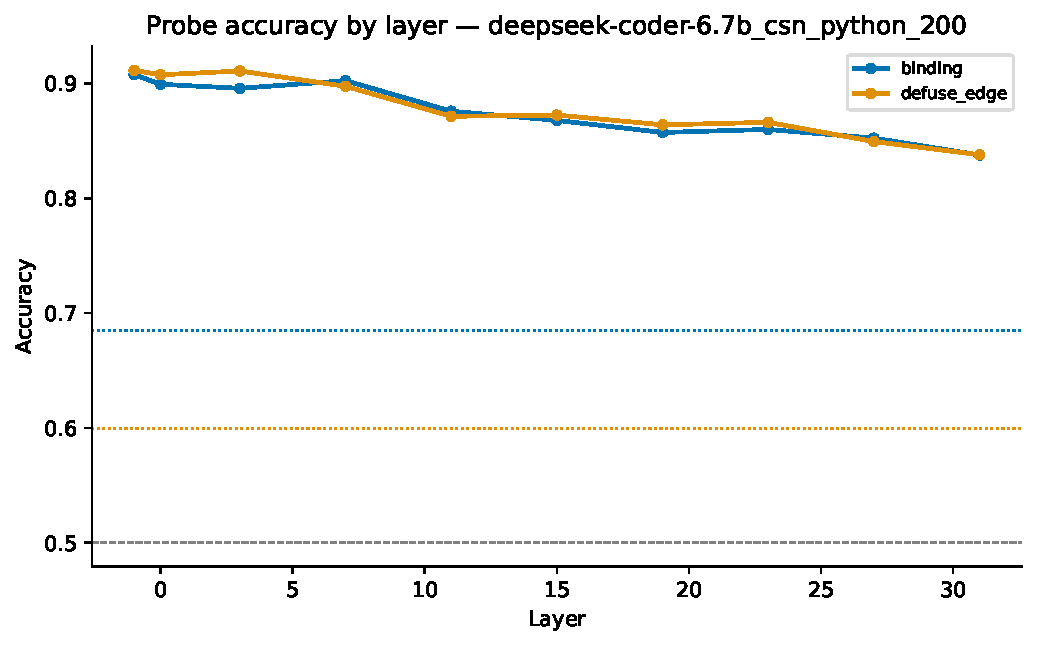
\includegraphics[width=\linewidth]{layers_accuracy_deepseek-coder-6.7b_csn_python_200.pdf}
    \caption{Accuracy by layer.}
  \end{subfigure}
  \hfill
  \begin{subfigure}[t]{0.49\linewidth}
    \centering
    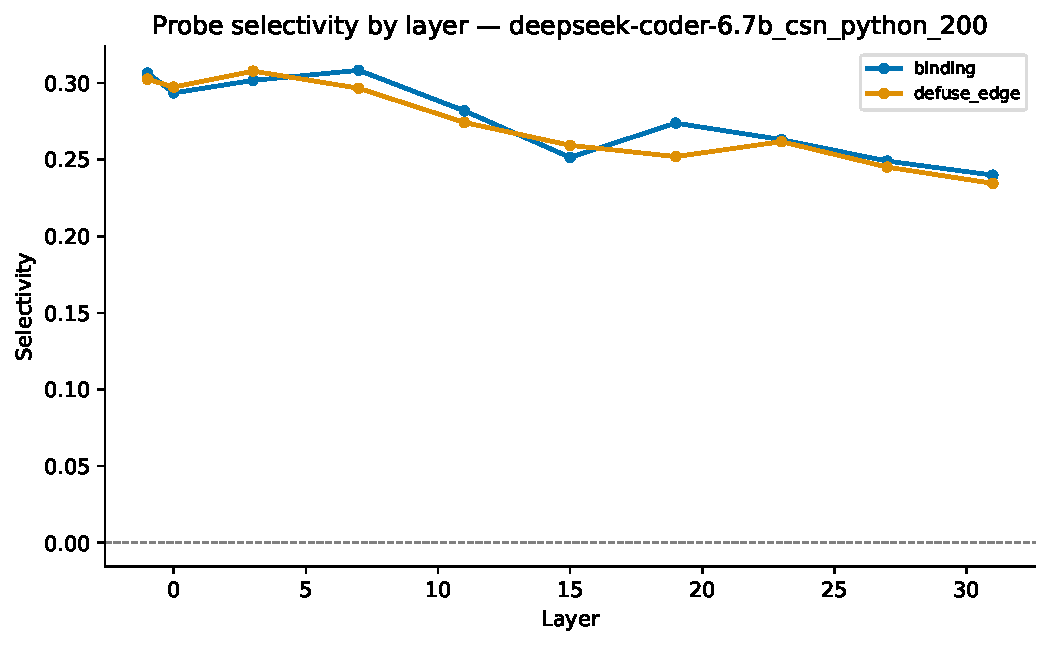
\includegraphics[width=\linewidth]{layers_selectivity_deepseek-coder-6.7b_csn_python_200.pdf}
    \caption{Selectivity by layer.}
  \end{subfigure}
  \caption{Real-code transfer in 6.7B. The early-middle peak and late decline resemble the synthetic results, but natural lexical cues make the embedding state informative.}
  \label{fig:real-code}
\end{figure}

\subsection{Context and semantics-preserving transformations}

Table~\ref{tab:context} gives layer-averaged frozen-probe accuracy at selected context sizes. Comment prose mainly changes distance; scope shadowing adds new uses of the tracked names in nested scopes. Their widening gap shows that semantic interference, rather than length alone, is the dominant failure mode. The main text quotes the best-layer comment result at 500 tokens (0.921); the table reports the all-layer average (0.914), which is why the values differ slightly.

\begin{table}[h]
  \centering
  \small
  \caption{DeepSeek-Coder 6.7B frozen-probe accuracy under added context, averaged over evaluated layers. Sources: \texttt{context\_degradation\_deepseek-coder-6.7b.csv}.}
  \label{tab:context}
  \begin{tabular}{llrrrr}
    \toprule
    Task & Filler & 0 tokens & 100 & 500 & 1,000 \\
    \midrule
    Binding & Comment prose & 0.974 & 0.922 & 0.914 & 0.902 \\
    Binding & Dead code & 0.974 & 0.908 & 0.786 & 0.759 \\
    Binding & Lexical decoy & 0.974 & 0.877 & 0.797 & 0.769 \\
    Binding & Competing update & 0.975 & 0.854 & 0.862 & 0.844 \\
    Binding & Scope shadow & 0.974 & 0.745 & 0.576 & 0.519 \\
    \midrule
    Def--use & Comment prose & 0.980 & 0.908 & 0.892 & 0.881 \\
    Def--use & Scope shadow & 0.981 & 0.722 & 0.643 & 0.596 \\
    \bottomrule
  \end{tabular}
\end{table}

The obfuscation ladder in Table~\ref{tab:obfuscation} is cumulative. \emph{Rename} consistently changes local identifiers; \emph{opaque} adds provably dead branches; \emph{encode} rewrites arithmetic; and \emph{flatten} replaces structured control flow with a dispatch loop. Every program variant is execution-verified against its base. The table averages over layers, so it hides the main layerwise result: after renaming, early layers fall below chance while middle layers remain at approximately 0.85--0.90. Flattening damages even the best layer.

\begin{table}[h]
  \centering
  \small
  \caption{DeepSeek-Coder 6.7B frozen-probe accuracy across the cumulative obfuscation ladder, averaged over layers. Source: \texttt{obfuscation\_robustness\_deepseek-coder-6.7b.csv}.}
  \label{tab:obfuscation}
  \begin{tabular}{lrrrrr}
    \toprule
    Task & Normalize & Rename & Opaque & Encode & Flatten \\
    \midrule
    Binding & 0.974 & 0.726 & 0.722 & 0.738 & 0.590 \\
    Def--use & 0.976 & 0.701 & 0.703 & 0.717 & 0.598 \\
    \bottomrule
  \end{tabular}
\end{table}

\begin{figure}[h]
  \centering
  \begin{subfigure}[t]{0.49\linewidth}
    \centering
    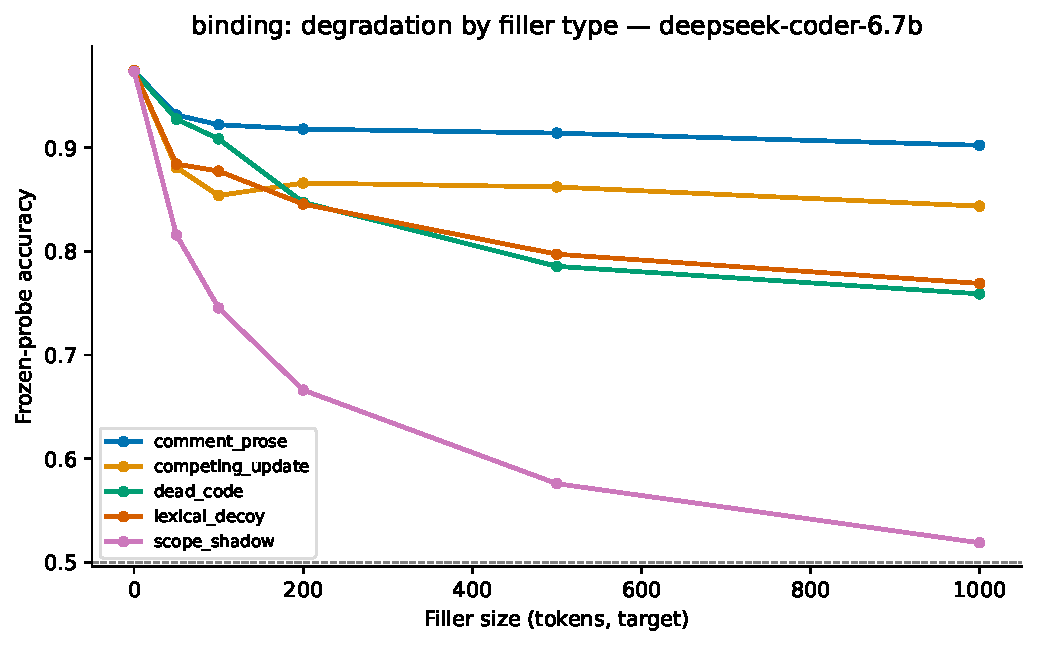
\includegraphics[width=\linewidth]{context_binding_deepseek-coder-6.7b.pdf}
    \caption{Inserted context.}
  \end{subfigure}
  \hfill
  \begin{subfigure}[t]{0.49\linewidth}
    \centering
    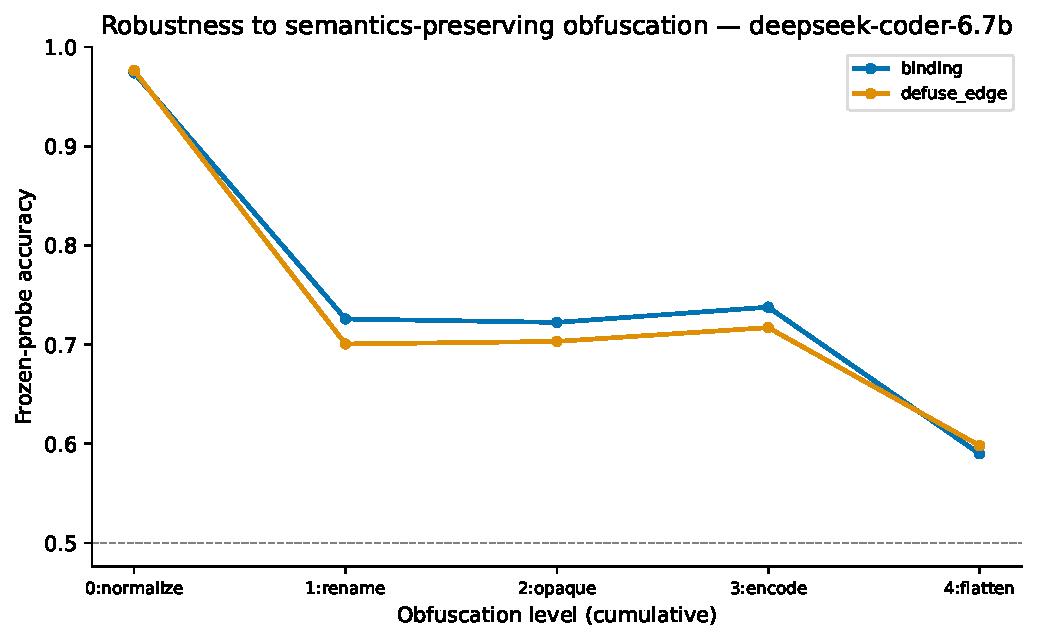
\includegraphics[width=\linewidth]{obfuscation_levels_deepseek-coder-6.7b.pdf}
    \caption{Obfuscation ladder.}
  \end{subfigure}
  \caption{Robustness of the accessible relation. Inert length is comparatively inexpensive; scope interference and flattened control structure are the clear limits.}
  \label{fig:robustness-appendix}
\end{figure}

\subsection{Cross-scale causal routing}

Table~\ref{tab:patching-replication} reports the smaller-model replication omitted from the main figure. Recovery can exceed one when a patch moves the answer beyond the clean endpoint; it should be read as normalized effect size, not probability. The qualitative result matches 6.7B: causal influence begins at the sink argument, moves to the final position, and is absent at the sanitizer-definition position.

\begin{table}[h]
  \centering
  \small
  \caption{Selected activation-patching results for DeepSeek-Coder 1.3B. Source: \texttt{causal\_patching\_summary\_deepseek-coder-1.3b.csv}.}
  \label{tab:patching-replication}
  \begin{tabular}{rrrr}
    \toprule
    Layer & Sink argument & Final token & Sanitizer definition \\
    \midrule
    $-1$ & 0.000 & 0.000 & 0.000 \\
    0 & 1.087 & 0.107 & 0.000 \\
    3 & 0.872 & 0.129 & 0.000 \\
    7 & 0.208 & 0.561 & 0.000 \\
    11 & 0.106 & 0.771 & 0.000 \\
    19 & 0.095 & 0.899 & 0.000 \\
    23 & 0.000 & 1.000 & 0.000 \\
    \bottomrule
  \end{tabular}
\end{table}

\subsection{Jacobian-lens implementation validation}

Table~\ref{tab:jlens-validation} shows selected next-token validation layers. Top-1 is the fraction of examples on which the correct held-out identifier is ranked first; MRR is the mean reciprocal rank of that identifier. The Jacobian lens substantially exceeds random directions and improves on the plain logit lens at several pre-final layers. Equality of Jacobian and logit results at layer 31 is required by the closed-form identity check, not an empirical coincidence.

\begin{table}[h]
  \centering
  \small
  \caption{Selected 6.7B next-token validation results ($n=60$ per cell). Source: \texttt{jlens\_validation\_deepseek-coder-6.7b.csv}.}
  \label{tab:jlens-validation}
  \begin{tabular}{rrrrrrr}
    \toprule
    & & \multicolumn{2}{c}{J-lens} & \multicolumn{2}{c}{Logit lens} & \multicolumn{2}{c}{Random} \\
    \cmidrule(lr){3-4}\cmidrule(lr){5-6}\cmidrule(lr){7-8}
    Layer & Top-1 & MRR & Top-1 & MRR & Top-1 & MRR \\
    \midrule
    3  & 0.283 & 0.465 & 0.150 & 0.243 & 0.000 & 0.139 \\
    15 & 0.300 & 0.452 & 0.183 & 0.339 & 0.017 & 0.107 \\
    19 & 0.567 & 0.662 & 0.383 & 0.542 & 0.033 & 0.157 \\
    27 & 0.650 & 0.752 & 0.650 & 0.759 & 0.017 & 0.130 \\
    31 & 0.517 & 0.706 & 0.517 & 0.706 & 0.000 & 0.116 \\
    \bottomrule
  \end{tabular}
\end{table}

\section{Retired Analyses, and Why}
\label{app:retired}

Three claims from an earlier version of this work are withdrawn. We keep their measurements here because the reasons they failed are the paper's methodological content, and because a reader is better served by seeing which controls did the retiring than by seeing only the results that survived. All underlying data remain in the repository and every analysis below is reproducible from it.

\paragraph{A null whose positive control was of the wrong kind.}
We reported that control dependence is decodable (probe AUC 0.999) but not available to an output-aligned readout: at guard anchors, a Jacobian lens ranked the guard's own variable at 0.813 while the control-dependence target stayed at chance at every layer. The measurement stands, including a temporal confound we found and removed (Table~\ref{tab:temporal-control}); after correction, 0.500 lies inside every program-clustered interval. What does not stand is the interpretation. The positive control asks the readout to name a variable that is present at the anchor --- an identity fact. The test asks it to name a variable standing in a \emph{relation} to the anchor. A readout that can express the first and not the second is not evidence that the model lacks the relation; it may be evidence that this readout cannot express relations at these positions, and nothing in the design separates those. A second intended control failed for a mechanical reason: the guard anchor is the trailing literal of the guard expression, so the ``next identifier'' is several tokens downstream past the colon and the indent.

\paragraph{A metric that rewarded unreliability.}
We reported that a taint probe remains correct at the prefixes where the model answers wrongly, and that no anticipatory degradation survives a floor. The first half is a measurement and it holds. The second half rested on an early-warning statistic that we now know is not fit for the purpose: within a family of readouts, the apparent warning rate is almost perfectly predicted by how often the readout is simply wrong, so an uninformative direction scores well by erring early and often. Table~\ref{tab:leadtime} shows a model-free position rule scoring $+0.113$ against a 99\%-accurate probe's $-0.010$. A metric that cannot distinguish anticipation from unreliability does not become trustworthy when it returns a null, so we report neither direction. The original positive result, prior to these floors, was measured on a prompt under which both models emitted a constant answer (balanced accuracy exactly 0.500, Table~\ref{tab:behavior-sanity}); their opposite response biases manufactured an apparent difference between scales.

\paragraph{A causal claim whose intervention transported the input.}
We reported that patching the sanitizer-definition position recovers nothing, and read this together with the probe result as showing that the model represents sanitization without routing it to the answer. The recovery numbers stand and are reported in Section~\ref{sec:causal}; the reading does not, for the reasons given there. The relevant failure is that the design's informative position is also the only position at which the two programs differ.

The common thread is that all three were claims about \emph{absence}, and absence is the hardest thing to establish. Each needed a positive control matched in kind to the test, at the same site, on the same states; none had one.

\subsection{Control-dependence readout and its temporal control}

The control-dependence comparison initially mixed candidates on opposite sides of the guard anchor. Table~\ref{tab:temporal-control} shows the corrected subset in which both candidates occur after the anchor. Accuracy remains close to the exact 0.500 chance level throughout. The main-text positive control is evaluated separately because it asks which variable is present in the guard, rather than which later statement depends on it.

\begin{table}[h]
  \centering
  \small
  \caption{Temporally matched 6.7B J-lens control-dependence accuracy ($n=415$ per layer). Source: \texttt{jlens\_controldep\_summary\_deepseek-coder-6.7b.csv}.}
  \label{tab:temporal-control}
  \begin{tabular}{rrrrrrrrrr}
    \toprule
    Layer & $-1$ & 0 & 3 & 7 & 11 & 15 & 19 & 23 & 31 \\
    \midrule
    Accuracy & 0.480 & 0.535 & 0.484 & 0.472 & 0.448 & 0.472 & 0.472 & 0.494 & 0.504 \\
    \bottomrule
  \end{tabular}
\end{table}

\subsection{Behavioral-signal validation and the early-warning audit}

The forced-choice behavior is useful only if the model distinguishes tainted from untainted prefixes. Table~\ref{tab:behavior-sanity} reports both raw and balanced accuracy. Balanced accuracy is the mean recall over the tainted and untainted classes, so a constant responder scores 0.500 regardless of class imbalance. This is why 6.7B supports a lead-time analysis and 1.3B does not.

\begin{table}[h]
  \centering
  \small
  \caption{Behavioral-signal validation. Sources: \texttt{behavioral\_sanity\_*.csv}.}
  \label{tab:behavior-sanity}
  \begin{tabular}{lrrrrl}
    \toprule
    Model & Prefixes & Accuracy & Balanced acc. & Says tainted & Usable \\
    \midrule
    1.3B & 342 & 0.629 & 0.471 & 0.734 & No \\
    6.7B & 342 & 0.939 & 0.836 & 0.874 & Yes \\
    \bottomrule
  \end{tabular}
\end{table}

For a readout with per-prefix error rate $\epsilon$, the analytic null is the probability that independent readout errors occur before the model's first error. Early-warning excess is observed early-warning rate minus this null. Table~\ref{tab:leadtime} reports representative 6.7B layers. At layers 0, 7, 19, 23, and 27, the probe makes almost no prefix errors and never fails before the model; in all 19 model-wrong examples it is correct at every prefix. Layer 15 has a small positive excess but does not survive correction across layers. Layer 31 is less reliable and therefore produces a larger apparent warning, illustrating why the analytic floor is necessary.

\begin{table}[h]
  \centering
  \small
  \caption{Representative corrected lead-time results for 6.7B. ``Never wrong'' counts model-wrong examples for which the readout remains correct at every prefix; the denominator is 19. Source: \texttt{behavioral\_leadtime\_summary\_deepseek-coder-6.7b.csv}.}
  \label{tab:leadtime}
  \begin{tabular}{rlrrrr}
    \toprule
    Layer & Readout & Prefix error & Warning rate & Excess & Never wrong \\
    \midrule
    all & Position only & 0.233 & 0.842 & 0.113 & 3 \\
    0  & Probe & 0.005 & 0.000 & $-0.024$ & 19 \\
    7  & Probe & 0.008 & 0.000 & $-0.041$ & 19 \\
    11 & Probe & 0.027 & 0.105 & $-0.023$ & 17 \\
    15 & Probe & 0.013 & 0.211 & 0.149 & 13 \\
    19 & Probe & 0.014 & 0.000 & $-0.069$ & 19 \\
    23 & Probe & 0.016 & 0.000 & $-0.080$ & 19 \\
    27 & Probe & 0.010 & 0.000 & $-0.049$ & 19 \\
    31 & Probe & 0.172 & 0.789 & 0.183 & 4 \\
    \bottomrule
  \end{tabular}
\end{table}

\begin{figure}[h]
  \centering
  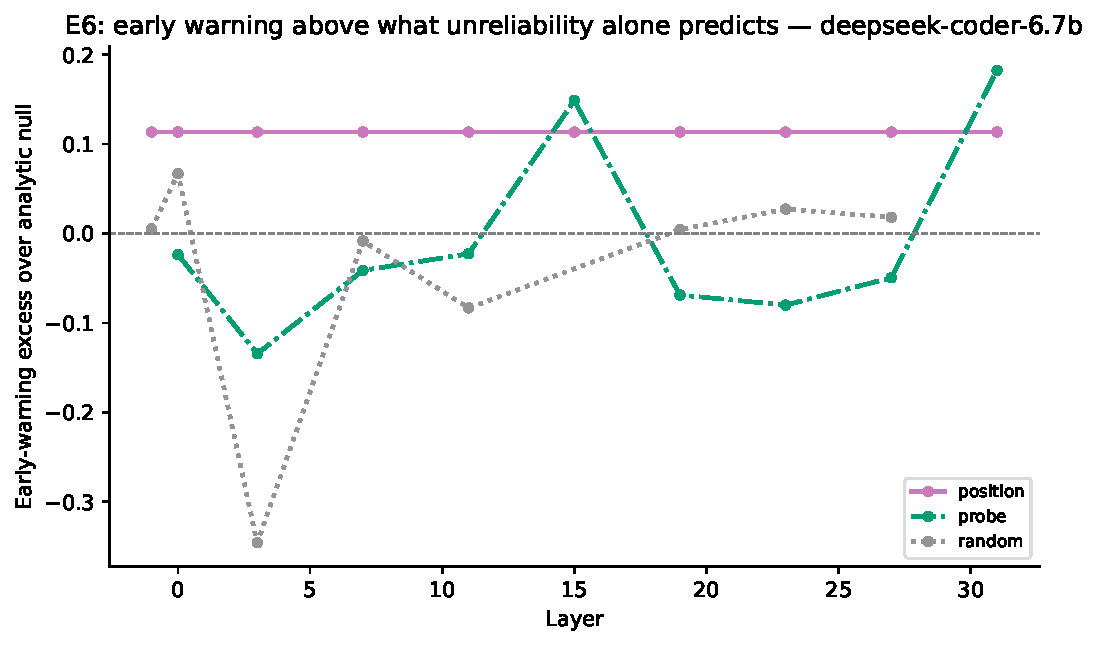
\includegraphics[width=0.7\linewidth]{leadtime_excess_deepseek-coder-6.7b.pdf}
  \caption{Early-warning excess after accounting for each readout's error rate. The position-only baseline exceeds the reliable probe at most layers; degraded or random readouts can appear more anticipatory because they make more errors.}
  \label{fig:leadtime-audit}
\end{figure}

\section{Reproducibility Notes}
\label{app:reproducibility}

The canonical configuration uses seed 42. Activation extraction is separated from probe fitting, and every paper table and figure is regenerated from the CSV files alone by \texttt{scripts/90\_make\_paper\_assets.py}. Run manifests record command-line arguments and git revisions. The repository also contains tests for data generation, graph extraction, token alignment, probe construction, the Jacobian-lens calculation, and independent ground-truth cross-checks.

\bibliographystyle{plainnat}
\bibliography{references}

\end{document}
